% Andrew G. West - prop_spec.tex
% Main LaTeX file for CIS400/401 Project Proposal Specification
%

\documentclass{sig-alternate}
 
\usepackage{mdwlist}
\usepackage{url}
\usepackage{graphicx}
\usepackage{float}
\usepackage[section]{placeins}
\begin{document} 

\title{BERTRAM: A Bartending Robot}

\subtitle{Dept. of CIS - Senior Design 2011-2012}
\numberofauthors{3}
\author{
\alignauthor Seth Shannin \\ \email{sshannin@seas.upenn.edu} \\ Univ. of Pennsylvania \\ Philadelphia, PA
\alignauthor Kevin Xu \\ \email{kevinxu@seas.upenn.edu} \\ Univ. of Pennsylvania \\ Philadelphia, PA
\alignauthor Dr. Camillo Jose Taylor \\ \email{cjtaylor@cis.upenn.edu} \\ Univ. of Pennsylvania \\ Philadelphia, PA}
\date{}
\maketitle

\begin{abstract}
\textit{\indent Programming a robot to autonomously perform human tasks has been a 
long-time goal of robotics. Such endeavors have typically involved heavy 
computation due to the demands of visual processing, path planning, and motor 
coordination. Human demonstration has often been used to introduce a sequence 
of moves to a robot, in the form of both inverse kinematics (direct physical 
manipulation of the robot's limbs) and visual observation. Here we 
investigate teaching robotic motion through the development of an immersive
teleoperation system for controlling the PR2. Unlike previous attempts to
control the PR2 from a distance (`teleoperation'), we propose to also provide the
operator with an `immersive' experience by allowing the operator to experience 
the environment from the robot's perspective. \\
\indent We plan to evaluate the effectiveness of the system
by attempting to mix and serve drinks with a Willow Garage PR2 
humanoid robot controlled by a user of this immersive teleoperation system. Following the implementation of this system, we will evaluate how it can be used to allow
the PR2 (or any robot for that matter) to rapidly acquire new behavior within a specific environment. If successful, we will have demonstrated a novel and natural method for a
human operator to impart a specific movement sequence to a robot. This paper details our progress in regards to implementing the immersive teleoperation system and our plans to use it to teach PR2.}
\end{abstract}

\section{Introduction}
\label{sec:intro}
\indent Constructing a fully autonomous and adaptive robot is one of the more
elusive goals of robotics research.
The possibility of a robotic butler is only one of many potential applications. However, true
autonomous decision making (that is, free of direct control from a human operator) is an incredibly challenging process as many different systems must 
be coordinated to make this possible. For instance, visual information must be processed quickly and accurately to respond to 
changes in the environment, accurate path planning is needed to navigate the environment, and 
precise motor coordination is needed to manipulate the environment. There have been many different 
attempts at overcoming these challenges involved in developing an autonomous robot. \\
\indent One major type of approach 
that has been often explored involves the field of machine learning. The ability to learn can be a powerful intermediate 
step towards autonomy, since learning can allow a robot to adapt to new, unforeseen scenarios on its own. 
Teaching by human demonstration is a common approach to robot learning because it enables the 
transmission of complex behavior in a manner far easier than individually planning the movement of each motor and joint. However, choosing exactly how the demonstrated behavior is delivered to the 
robot in such a way that it can record and reproduce that behavior is still a very challenging task.\\ 
\indent In this paper we report on our progress towards teaching the WillowGarage PR2 Robot to mix and
serve drinks by first implementing an immersive teleoperation system for controlling the PR2. By `teleoperation', we simply mean controlling the PR2 from
a distance. By `immersive', we mean giving the human operator the illusion of being inside the PR2. The PR2 is a humanoid robot developed by  Willow Garage~\cite{pr2} for the purpose of robotics 
research. It is omnidirectional and capable of telescoping height. What makes the PR2 especially attractive for robotics research is its pair of highly movable arms and grippers that allow grasping of many different kinds of objects. The PR2 also comes with a robust series of highly useful software development tools,
including a versatile simulator that allows developers to perform trial runs on a virtual PR2 without
risking damage to the actual robot or environment. Institutions across the
world have taught the PR2 a wide variety of human actions, such as baking 
cookies~\cite{cookies}, scanning and bagging groceries~\cite{groceries}, and fetching a sandwich from 
Subway~\cite{subway}. However, unlike in these examples, we propose to teach the PR2 a new behavior not through advanced task planning, but rather through human
demonstration. Thanks to the University of Pennsylvania's GRASP laboratory, we have access to a real PR2 (shown in Figure~\ref{fig:pr2_photo}) that we can use to test the implementation of our system.\\
\begin{figure}[htb] 
	\begin{center}
		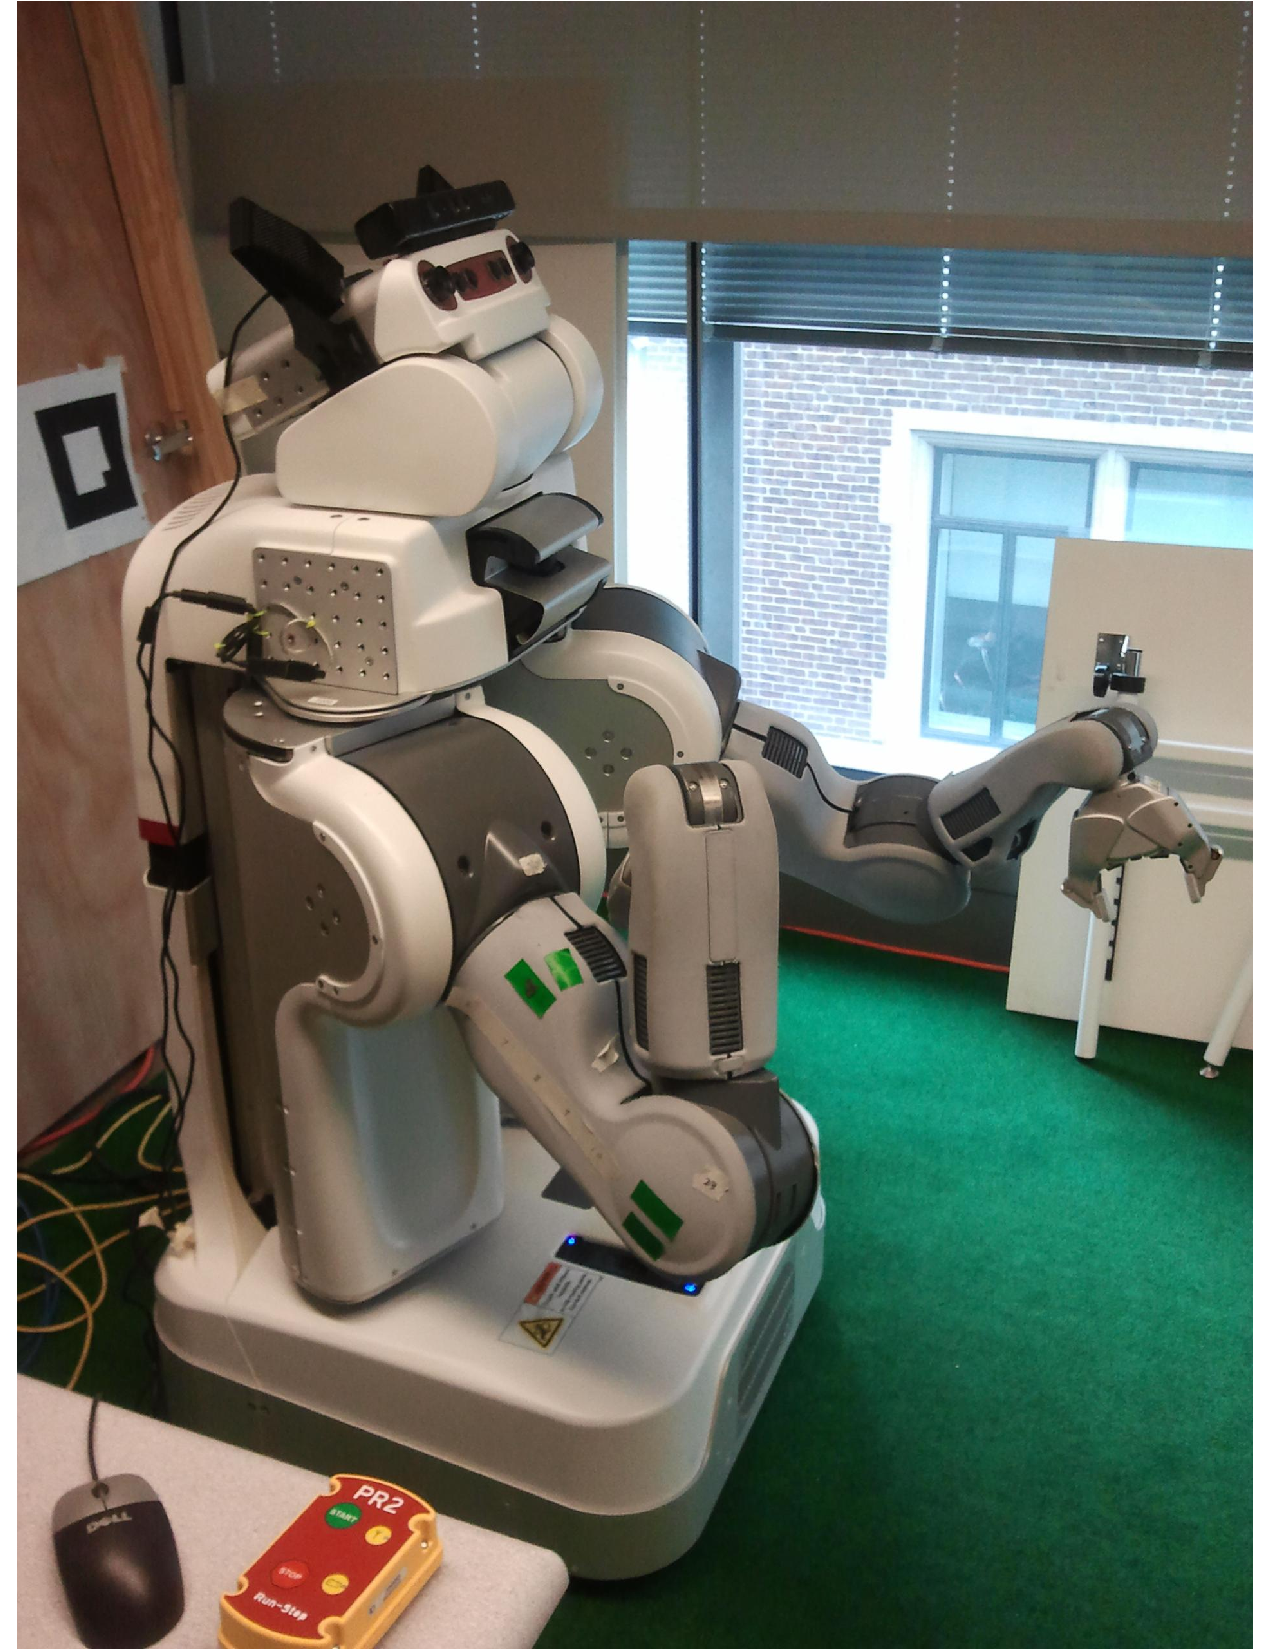
\includegraphics[width=0.75\linewidth]{graspy}
	\end{center}
	%\vspace{-24pt}
	\caption{PR2 robot at the University of Pennsylvania, nicknamed `GRASPY'}
	\label{fig:pr2_photo}
\end{figure}
\indent The chief component of our teleoperation system is the Microsoft XBox Kinect sensor. This sensor provides depth information at real-time speeds
(30 frames per second), which essentially performs the computation that would have been required for stereo 
processing. Combined with various open source libraries~\cite{kinect}, the Kinect also works with 
software that provides human motion sensing and tracking, which greatly simplifies the task of capturing human body movements.
These Kinect libraries have already been used successfully in 
many projects involving real-time tracking of human motion, examples of which can be found online~\cite{freenect}.\\
\indent We propose to use the Kinect as part of an immersive teleoperation system to teach the PR2 how to mix and pour different kinds of drinks.
The Kinect sensor provides a convenient way to capture a human demonstration of desired behavior. The captured data can be relayed to the
PR2 via ROS, an open-source Robot Operating System\cite{ros}. ROS provides a 
convenient framework for device abstraction and inter-process communication. 
Processes that perform computation are visualized as nodes in a graph, with inter-process communication representing the
edges of the graph. Nodes send information to each other in the form of messages. Nodes that wish to send messages to other nodes can
`publish' to a topic, and nodes wishing to receive these messages need only to `subscribe' to these topics. ROS enables relatively short
programs to issue surprisingly sophisticated commands to the PR2, such as moving all of the arm joints to a specific position within a
specified time frame. By using ROS along with the PR2 and the Kinect, we will construct a system for operating the PR2 remoting while
giving the operator the feeling of being within the robot itself. The effectiveness of this system in teaching the PR2 new tasks will then be evaluated.

What follows is an overview of other work related to implementing of 
teleoperation systems and teaching robots human-like tasks. We then describe 
the components of our proposed immersive teleoperation system before delving 
into the technical implementation of each component. After this is an 
evaluation of the current performance of the system and a summary of remaining work.

\section{Related Work}
\label{sec:related_work}
\indent There have been many previous teleoperation implementations for robotic systems. Kofman \textit{et al.}~\cite{robot_interface} devised a system for controlling a robotic arm via teleoperation and sending visual feedback to the user. The setup used in their work involves multiple cameras aimed at the human operator to capture 3-D information about the operator's arm movements. This data is then sent to a remote site containing the robotic arm and mapped to its joints so it can mimic the motion of the human arm. The human operator is able to see the robotic arm via cameras positioned at the remote site that send visual feeds of both the entire arm and of vision from the point of view of the tip of the robotic arm. Fortunately for us, the Kinect, when paired with ROS, provides a much simpler and less complicated setup to capture arm motion and send them to the PR2's arm. We are far from the first to implement teleoperation of a robot via the Kinect and ROS. In fact, Willow Garage has already tried integrating Kinect with ROS to control the PR2 remotely~\cite{willow_kinect}. However, our ultimate goal includes not only developing an immersive teleoperation system for the PR2, but also investigating how this system can be used to teach the PR2 new behavior, such as mixing and serving drinks.

Other institutions have conducted research involving autonomous robots handling
drinks. Hillenbrand \textit{et al.}~\cite{pouring_arm} designed a 
semi-autonomous hand-arm robot for this purpose. The hand-arm was capable of 
responding to user input by choosing a drink from a variety of different 
containers, opening the drink if necessary, pouring the liquid into a glass, 
and then offering the cup to the user. It was capable of not only picking up 
bottles and cups, but also of unscrewing bottle caps. Processing of visual data
from cameras was combined with object recognition to identify the drinks, after
which grasp planning was used to actually pick up and manipulate the drink. 
Srinivasa \textit{et al.}~\cite{herb} designed an autonomous robot capable of 
navigating a household-like environment and manipulating a wide variety of 
everyday objects. Consisting of an arm mounted on a segway, HERB used a 
powerful array of six multi-core processors to successfully traverse its 
environment and interact with objects around it, such as cups and drawers. By 
combining different processes for object recognition, task based planning, and 
caged grasping, HERB was able to autonomously carry out commands issued from a 
graphical user interface to perform simple kitchen tasks, such as placing an 
object in a recycling bin or lifting a mug. The teaching approach taken by both
of these works relies primarily on heavy amounts of computation to carefully 
plan each action that the robot will execute ahead of time.  The chief 
difference in our system is that we intend to teach a robot to do these kinds
of things more quickly and naturally by first having a human operator of our 
teleoperation system execute the actions.\\
\indent There has also been substantial work done in teaching the PR2 robot to perform various human tasks. Bohren \textit{et al.}~\cite{beer} used the PR2 and ROS to build a robotic system for retrieving a beer from a refrigerator. In their work, they developed a task-level execution system for rapidly prototyping different robotic applications. The PR2 had to navigate an obstacle map to reach the refrigerator, use object recognition and grasp planning to identify the door handle and the drinks, and ultimately use facial recognition to deliver the beer to a human recipient. Each step of the process contained detail planning and image processing in order to carry out the expected behavior. Klingbeil \textit{et al.}~\cite{groceries} developed a grasping algorithm to enable the PR2 to pick up objects and attempt to locate and scan the barcode. Their technique allowed the PR2 to devise a plan to grasp the object from only a single 3D snapshot. Their algorithm emphasized the importance of positioning the PR2's gripper such that its shape most closely matched the shape of the object it attempts to grasp. Saito \textit{et al.}~\cite{subway} devised a way for the PR2 to intelligently navigate large environments via semantic search. The PR2 attempts to find a specific object by first searching areas that would logically contain that item. When asked to retrieve a sandwich, the PR2 first inspected a nearby refrigerator in its environment. If it fails to find one there, it then determines the next most likely place a sandwich could be found. These approaches to teaching the PR2 emphasize complex algorithms used to enable the PR2 to devise a plan from scrach to act autonomously in a given environment. Our approach is simpler in that we plan to use recorded input data from our immersive teleoperation system to give the PR2 a general sequence of actions to follow that can later be refined through more complex learning techniques.\\ 
\indent There have also been other approaches involving data from human demonstration to allow a robot to perform specific tasks. In a relatively early attempt, Chalodhorn \textit{et al.}~\cite{walk_imitation} used motion capture to teach a bipedal humanoid robot how to walk by imitation. Joint angles obtained from motion capture data recorded from a human demonstrator wearing a motion capture suit were mapped to joint angles on the robot. This data was combined with predictions based on sensory information to reproduce a human-like gait in the robot. Kormushev \textit{et al.}~\cite{whiteboard} taught a robot new motor skills through kinesthetic teaching, which is teaching by physical contact. The robot had two distinct modes of operation: a learning phase and a reproduction phase. First, the robot was shown how to clean a whiteboard by direct human manipulation of the robot's joints, recording both position and force information. Subsequently, the robot would translate the learned information to its own frame of reference and attempt to duplicate the teacher's movement pattern on the whiteboard.  Kormushev \textit{et al.}~\cite{pancakes} also used kinesthetic learning to teach a robotic arm how to flip a pancake. A human teacher first moved the arm to demonstrate the movement required to flip a pancake 180 degrees in the air and catch it again. In subsequent trials, reinforcement learning techniques were applied such that the robot could evaluate the performance of its flips and attempt to adjust the motion of the arm for better future flips.\\
\indent Our method has several advantages over these existing approaches. First of all, the Kinect sensor provides accurate real-time human
motion tracking that can be mapped to specific movement in the PR2 thanks to ROS. The Kinect also provides motion capture without the need
of complicated setups involving motion capture suits or multiple cameras. Secondly, an immersive scheme for controlling the robot
enables a human operator to more naturally move the robot in a given situation compared to manipulating the robot directly by physical
contact or through a joystick-based control scheme. Immersive teleoperation also enables direct control of robots that cannot be easily
subject to demonstration through physical contact, such as very large or very small robots. Our method, if successful, would allow for rapid demonstration of different sequences of behavior to the PR2, which could be stored and queued up for later reproduction and enhancement. This technique could be generalized to other humanoid robots besides the PR2 to teach them different kinds of behavior.

\section{System Model}
Specifically because a teleimmersive system is meant to be used by human 
operators to control a robot, the external/visible part of this
design must be simple. The number of devices used to get input from the user 
and to deliver feedback should be small, and these devices should require
minimal effort to use. To that
end, a good portion of the control data captured from the user is captured
passively. After the initial setup phase, the user should be able to control
the system with minimal effort; the system should just watch the user and
translate the user's movements into control instructions for the PR2.

To facilitate this process, we use a couple separate devices and some
fairly sophisticated software stacks. While the
devices mostly consist of cameras and accelerometers to track the user's 
motion, there are a couple button devices which allow the user to
perform non-humanoid operations on the robot (such as freezing a joint or
triggering certain routines).

The most obvious component of the system is the actual PR2 robot. This is the
device that user will be controlling by teleimmersive operation. The user must
be able to control each of the PR2's motors, including those for the head,
arms, hands, gripper, torso, and base of the robot. To make the teleoperation
immersive, the user will need have a direct feed from the PR2's onboard
camera system.

\begin{figure}[htb] 
	\begin{center}
		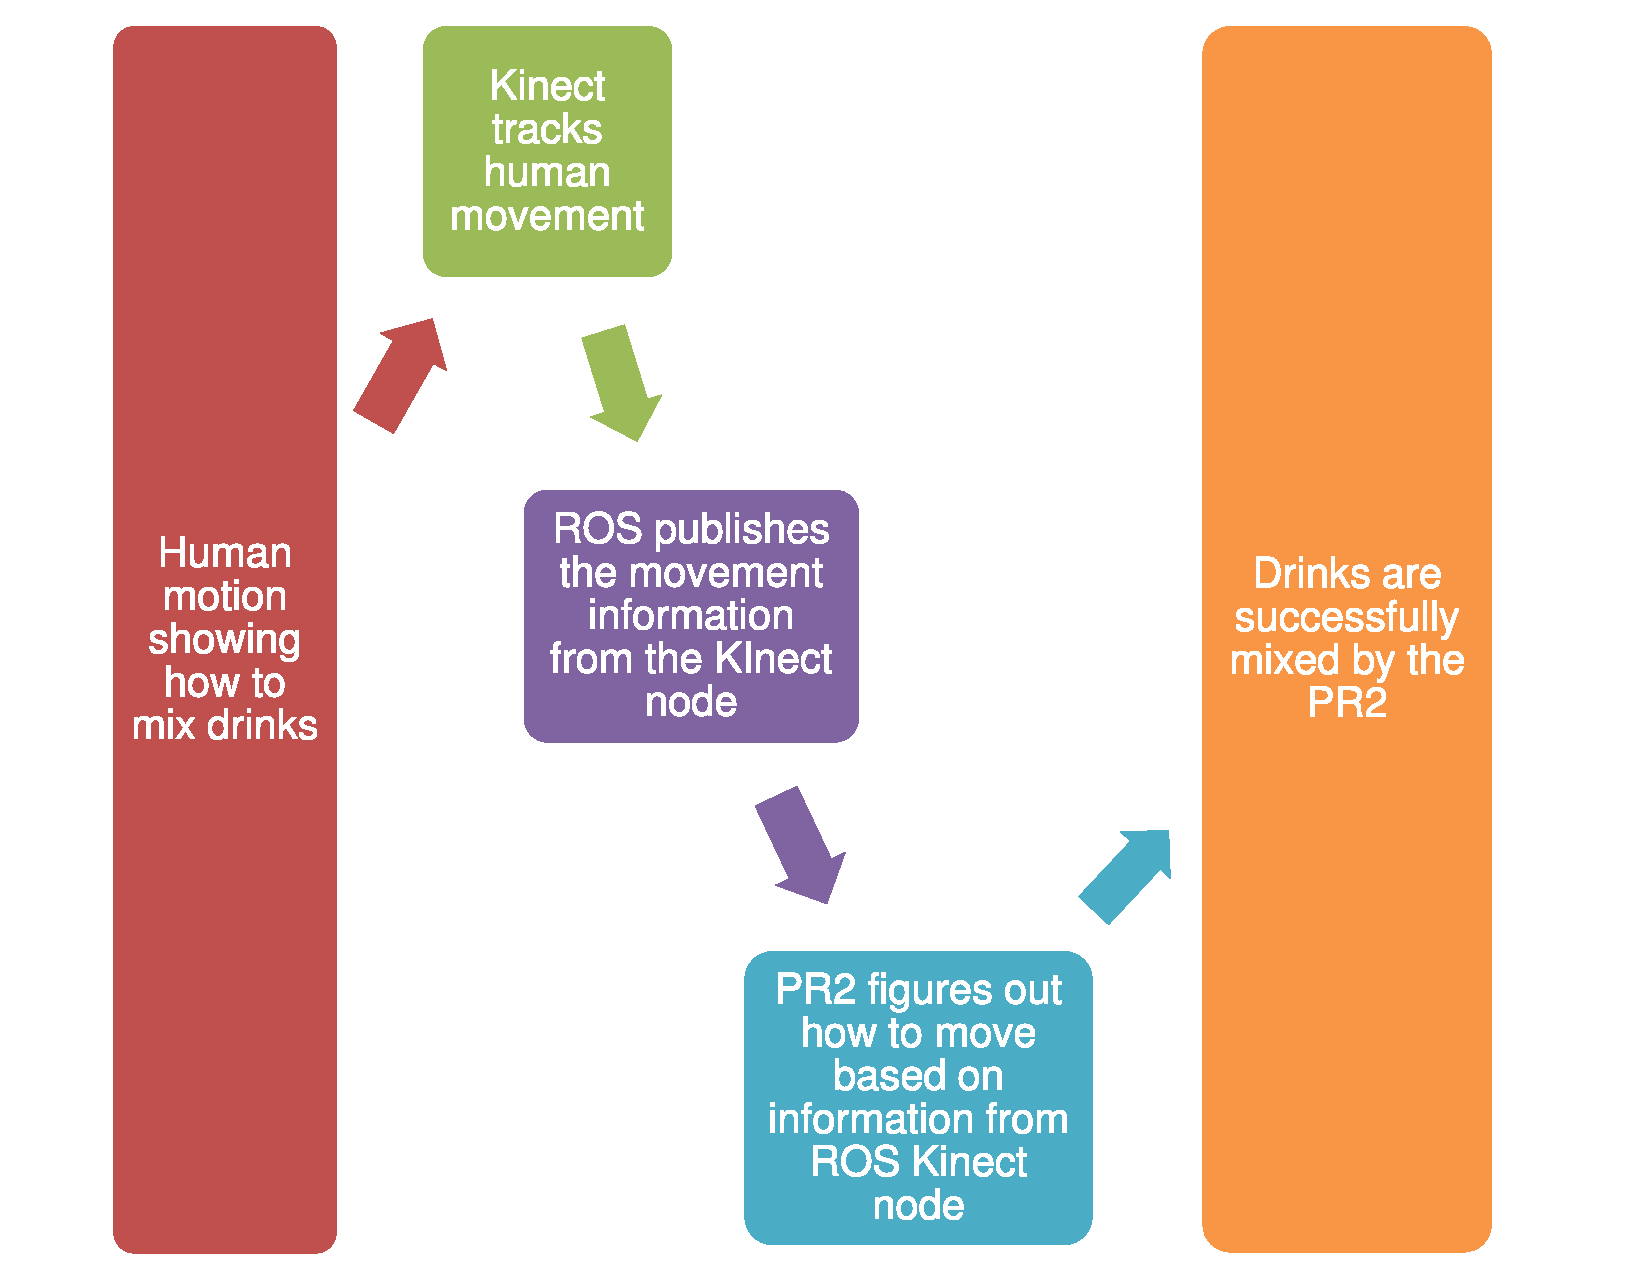
\includegraphics[width=1.0\linewidth]{flowchart}
	\end{center}
	%\vspace{-24pt}
	\caption{Block Diagram Summarizing System Model}
	\label{fig:some_graph}
\end{figure}


While the PR2 may be the most apparent aspect of the system,
the true nexus is ROS, the Robot Operating System. Although the
user will never need to interact explicitly with ROS, all communication between
the
user and the PR2 (in the form of commands or feedback) must pass through ROS.
ROS abstracts over devices and I/O, providing a common interface for accessing
any data stream or controlling any device. Using ROS, we can easily take
data from the many tracking devices, process all the data to come up with
movement plans for the PR2, and then actually command the PR2 to move in the
desired manner. This system architecture is shown Figure~\ref{fig:some_graph}.

Other than the PR2 robot itself, the Microsoft Kinect is perhaps the most 
prominent and obvious device in the teleimmersive operation system. The
hardware uses an 
infrared projector and stereo RGB cameras to create a 3D scene image complete
with depth information. It sends these raw video frames to ROS, which then
forwards the feed to a processing node. This processing node analyzes the 
video stream, identifies humanoid figures in the frames, and tracks these 
figures' joints. The Kinect does have some shortcomings though in that it does 
not reliably track wrist, finger, or head movements. We use separate 
accelerometer units to track these motions.

We capture wrist motion by having the user hold one Nintendo Wiimote with 
Wii MotionPlus in each hand. The Wiimote is a video game controller with 
multiple buttons, a direction pad, and built-in accelerometers. In this sense,
it is quite convenient. The user can comfortably hold one Wiimote in each hand,
(as this is how they were intended to be used in video games). The user now has
convenient access to a number of
control buttons and also is carrying accelerometers to track each of the wrist 
joints.

In order to track the user's head movements, we have the user wear a hat
with a three-axis accelerometer. This can track the yaw, pitch, and roll of the
user's neck joint and can therefore capture all head motions. The device is
approximately the size of a quarter and can be attached to any surface via
velcro.

The final hardware device is a pair of Vuzix augmented reality glasses.
Essentially, this is a pair of glasses with a mini LCD screen in each lens.
We take the video feed from the PR2's onboard stereo cameras and pipe it
directly into each eye. This is the immersive step which closes the loop and
helps place the user more fully into the system.

There is one other significant component to this system. This is the
component we have
termed in Figure~\ref{fig:some_graph} as the {\tt BERTRAM Analyzer}. This is a 
software node residing in ROS. Its primary function is to stitch together the
motion and position data from all the input devices (Kinect, Wiimotes, head 
IMU). It collates all the information and then maps the user's motions
into equivalent motions for the PR2.
\section{System Implementation}
Most of the interesting work in this project takes place inside the
{\tt BERTRAM Analyzer}, which collates all the captured motion data from the
user and processes this data to generate commands for the robot. ROS provides
bindings for both {\tt C++} and {\tt Python}. We chose to use Python due to our
familiarity with the language and due to the relative verbosity of {\tt C++}.
The analyzer registers for interrupt events from the Wiimotes and head-mounted
IMU and actively polls for Kinect events.

ROS interfaces with the Kinect using the {\tt openni} Kinect stack. The primary
function of this is to create a ROS node named {\tt openni\_tracker}. This
node identifies the Kinect device on a USB port and requests data
from it. It then attempts to identify people in the scene frame and start
tracking them. Once it has done so, it will publish data on various
topics (such as {\tt left\_shoulder}, {\tt right\_elbow}). These the messages
contain joint angle transforms and are delivered to the {\tt BERTRAM Analyzer}.

The {\tt BERTRAM Analyzer} listens to the messages from the
 {\tt openni\_tracker}.
When it receives information for an altered joint position, it applies the
appropriate transformations and instructs the PR2 on how to set its own joints
so as to mimic the sensed movement of the user. This is done for the shoulder
and elbow joints on both arms.

A similar process occurs for the head IMU. The specific IMU used is
the CHR-6dm Attitude and Heading Reference System. When lying flat, it uses
accelerometers to capture roll and pitch. It also has a magnetic compass to 
track yaw (necessary since the plane in which the yaw rotational motion occurs
is perpendicular to the gravity vector). After connecting to the 
controlling computer via 
USB, a ROS node is run to read in the data from the sensor and republish it
encapsulated in ROS messages. The {\tt BERTRAM Analyzer} is notified when these
messages are published. It reads the roll, pitch, and yaw data in the message
and sends the appropriate commands to the PR2. One feature which is not yet
implemented relates to the initialization of the IMU. Since it uses a compass
to track yaw, values are reported as angular deviations from magnetic north.
Therefore, when tracking a user who does not begin by facing north, it is 
important to find the unity position for the sensor (the bearing when 
the user is facing forward) and to use this as an offset for all future angle
readings.

The Wiimote communication is handled in much the same manner as the head IMU.
Instead of communicating via USB however, the Wiimotes communicate with the
controlling computer via Bluetooth. After the Wiimote pairs with the system,
ROS is used to create Wiimote node which 
sends a periodic stream of messages. Each message is a vector containing the
status of each button and sensor of the Wiimote. The {\tt BERTRAM Analyzer}
listens for these messages. It notes the state of each button it is watching
and takes the appropriate action (by sending commands to the PR2) if any are
pressed. Additionally, it reads in the accelerometer data. The Wiimote
provides only the actual angular velocities; it doesn't not translate the 
values into roll, pitch, or yaw positions. We therefore integrate these with respect to 
the publishing frequency to obtain an approximation of the actual roll, pitch,
and yaw angles for the wrist. Finally, the angles are translated into the PR2's
reference frame and then commands are sent instructing the PR2 to move. One 
item of note is that the human wrist rotates in only two degrees (that is,
the wrist does not rotate about the primary axis of the forearm). Although the PR2's 
gripper can actually rotate indefinitely in this axis, we instead map the 
rotation onto the forearm.

One nontrivial implementation detail to discuss is the physical method of
communication with the PR2. One option is to have the PR2's onboard computers
act as the controllers. Since this is a teleimmersive operation system, we find
this to be impractical, as the input devices may not be physically located
near the PR2. In addition, it is impractical to attach all these input devices 
directly to the PR2. The PR2 also contains multiple routers and hosts its
own wireless network. So far, this is the method we have used most when
communicating with the PR2 (for the sake of simplicity). In a real system however,
this manner of communication suffers from the same main problem as the first method: the user and devices
may be quite further away than a single WiFi source can reach. Fortunately,
the PR2 can also connect to and take IPs on other networks (communicating either by WiFi or by
Ethernet). Although we have so far run into complications when using this method, we
suspect these are due to issues with the computer we are using to control the
system rather than the PR2 itself.
In the long run, this is the method we intend to use when communicating with 
the PR2.

The final aspect of the system for which we need to discuss the implementation
is the visual feedback from the PR2 to the user. We accomplish this using a
pair of  Vuzix virtual reality goggles. The PR2 sends multiple image 
streams to ROS. As the goggles are not truly 3D, we intend to combine the left 
and right image feeds into one stream. This will then be sent to a node which will display the image
on the screen of the controlling computer. As the goggles accept a VGA input,
we can then simply connect them to the VGA video out port of the computer to
receive the image and display it to the user. We have tested this concept and
verified that it functions correctly using only a single camera source (such as
the left camera). All that remains is to combine the left and right camera
feeds together.
\section{System Performance}
We are currently in the process of completing the immersive 
teleoperation system using the components described in previous sections. Upon
completion, the system will be evaluated both for its ability to correctly
imitate the actions of a human operator as well as for its potential 
as a learning tool for the PR2 to acquire new behavior.\\
\subsection{Performance of Devices}
The PR2 has lived up to its expectations as a good choice of humanoid robot to 
use. Testing our existing code on the robot has been very straightforward, and 
the PR2 is fully capable of all of the arm motions, head motions, and grasping
we require it to do. ROS has also done an excellent job in allowing the 
{\tt BERTRAM Analyzer} to easily communicate back and forth with the diverse 
assortment of devices that comprise the teleoperation system.\\
\indent Capturing motion with the Kinect has been a painless process. It requires virtually no setup time and can transmit live human motion data in real time without the need for any special clothing or markers to indicate human joints or body parts. The user can more or less move freely once the Kinect has `calibrated' its view onto a target, which takes only a few seconds. ROS makes receiving the data from the Kinect very simple. Communication with the Wiimotes has also worked as expected. The remotes transmit their data wirelessly and accurately report button presses, rotations, and accelerations up to one hundred times per second. They fit nicely in the palms of the human operators' hands since they are originally intended to be used as video game controllers.\\
\indent The three-axis accelerometer for capturing head movement has been a little more difficult to deal with than originally anticipated. Although the device does report changes in its yaw, pitch, and roll, it is also prone to reporting errors if it receives sudden jolts or impacts. When these errors happen, the ROS software that interfaces with the device must be restarted to obtain accurate readings once more. We suspect that this problem will be alleviated once we mount it in a more stable fashion on to head gear for the human operator to wear. Ideally, the human operator can simply wear the head gear and not have to worr about adjusting the accelerometer. The video eyewear works as expected and can successfully display video output from cameras on the PR2.\\
\subsection {Performance of the BERTRAM Analyzer}
\indent The performance of the {\tt BERTRAM Analyzer} still needs to be improved. Although the physical devices that comprise our immersive teleoperation system are easy to use and are relatively few in number, the analyzer code has somewhat mixed performance in translating data from these devices into actions to the PR2. Although the PR2 does move its arms in accordance to the arms of the human operator, the arm movement is very abrupt and prone to sudden, uneven movements. This lack of precision in movement makes it difficult for the human operator to precisely control the arms to the degree needed to fine motions like lifting cups or glasses. We have tried to smooth out the arm motion by threshholding the values sent by the Kinect. In other words, we only send new actions to the PR2 if we receive data from the Kinect indicating that the human's arms have moved a certain amount from their previous positions. Although this change has made it easier to keep the PR2's arms still, it has not smoothed actual motions themselves. We are currently trying to address this issue by investigating how to limit the maximum acceleration and velocity of the PR2 arm motions.\\
\indent We have also run into some difficulty in mapping the rotation information from the Wiimote and three-axis accelerometer to the wrists and head of the PR2, respectively. The wrists and head do not always turn in a way that successfully imitates the wrist and head turns of the human operator. More work and experimentation with these components of the system need to be done before we can try and fix this problem.

\section{Remaining Work}
\label{sec:remaining_work}
\indent The most immediate goal is completion of the immersive teleoperation system. To achieve this, the arm movement of the PR2 needs to be smoothed out to allow fine-grained control. The wrist movement also must be improved to enable successful grasping of different objects. Once these two aspects of the PR2 are working well, additional work is required to correctly map head movement from the human operator to head movement of the PR2. This part is cruical for making the teleoperation feel immersive to the human operator of the system. Once the head motion is satisfactory, the human operator should be able to use the video eyewear to see from the PR2's perspective and operate the PR2 remotely without being in view of the actual robot. We estimate that we are currently about sixty percent done with the work needed to complete the immersive teleoperation system.\\
\indent Once this immersive teleoperation system is complete, additional work will be done to see how the system can be used to teach the PR2 new behavior. The idea is to repeat a specific action using the system and have the PR2 learn this behavior by recording the input data it receives. In this way, a human can demonstrate an action to the PR2, which will then enable the PR2 to repeat this action on its own. If enough time remains, methods to improve upon and refine this recorded behavior will be explored.

\subsection{Evaluation Critera}
\indent The performance of the immersive teleoperation system will
first be evaluated based on how well it can mimic the actions of
the human operator. We will attempt to grasp and lift a variety of
objects with the system to test the limits that the system allows in
controlling the actions of the PR2. The accuracy of the teleoperation
system can be measured with tests to determine with what level of precision
the arms of the PR2 move in relation to how much the arms of the human user move.\\
\indent Once the accuracy of the immersive teleoperation system has been verified, 
we can experimentally determining how quickly
and easily the PR2 can acquire new behavior from it. We will start
with very simple motions, such as simply lifting and pouring
a single cup or bottle. Once the PR2 is capable of completing
these actions on its own without the need of a human operator,
we can attempt to teach it increasingly complex sequences
of mixing and pouring. We can measure the PR2’s success
rate in repeating a recorded movement over multiple trials.
This success rate can be then be correlated with the complexity
of the demonstrated command. The goal here is to
show that many different movement sequences of varying
difficulty can be taught to the PR2 using the same motion
capturing setup from the Kinect.\\
\indent If time permits, we also plan to evaluate the PR2’s ability
to adapt its learned behavior to changing conditions. For instance, we can
measure how far a bottle can be moved from its expected
position before the PR2 becomes unable to pick it up. The
weight of the bottle can also be changed to see how well the
PR2 can adapt to grasping nearly-full versus nearly-empty
drink containers. The success rate of the PR2’s drink mixing
can be analyzed as a function of these variables (distance
moved, weight of drinks, etc).

\subsection{Timeline}
The following is a list of milestones we hope to reach as the spring semester progresses.
	% The 'itemize' environment shown here, and its friend 'enumerate' (shown below), are used to create indented\bulleted\outline style lists.
\begin{itemize*}
	\item {\sc prior-to Feb.1}: Achieve smooth arm and wrist motion on the PR2.\vspace{3pt}
	\item {\sc prior-to Mar.1}: Complete the immersive teleoperation system and attempt to mix drinks with the PR2.\vspace{3pt}
	\item {\sc prior-to Apr.1}: Teach the PR2 how to mix a drink using the completed system.\vspace{3pt}
	\item {\sc completion tasks}: Verify that the PR2 can successfully mix a drink, either autonomously or through human operation. Conduct accuracy testing. Complete write-up.\vspace{3pt}
	\item {\sc if there's time} : Investigate ways for the PR2 to improve behavior learned from the immersive teleoperation system.
\end{itemize*}

	% AW: We next move onto the bibliography.
\bibliographystyle{plain} % Please do not change the bib-style
\bibliography{progress_spec}  % Just the *.BIB filename

\end{document} 
